\RequirePackage{luatex85}
\documentclass[border={20pt,20pt,20pt,20pt}]{standalone}

\usepackage[dvipsnames]{xcolor}
\usepackage{tikz}
\usetikzlibrary{shapes, patterns, calc}

\def\angle{20}

\begin{document}
	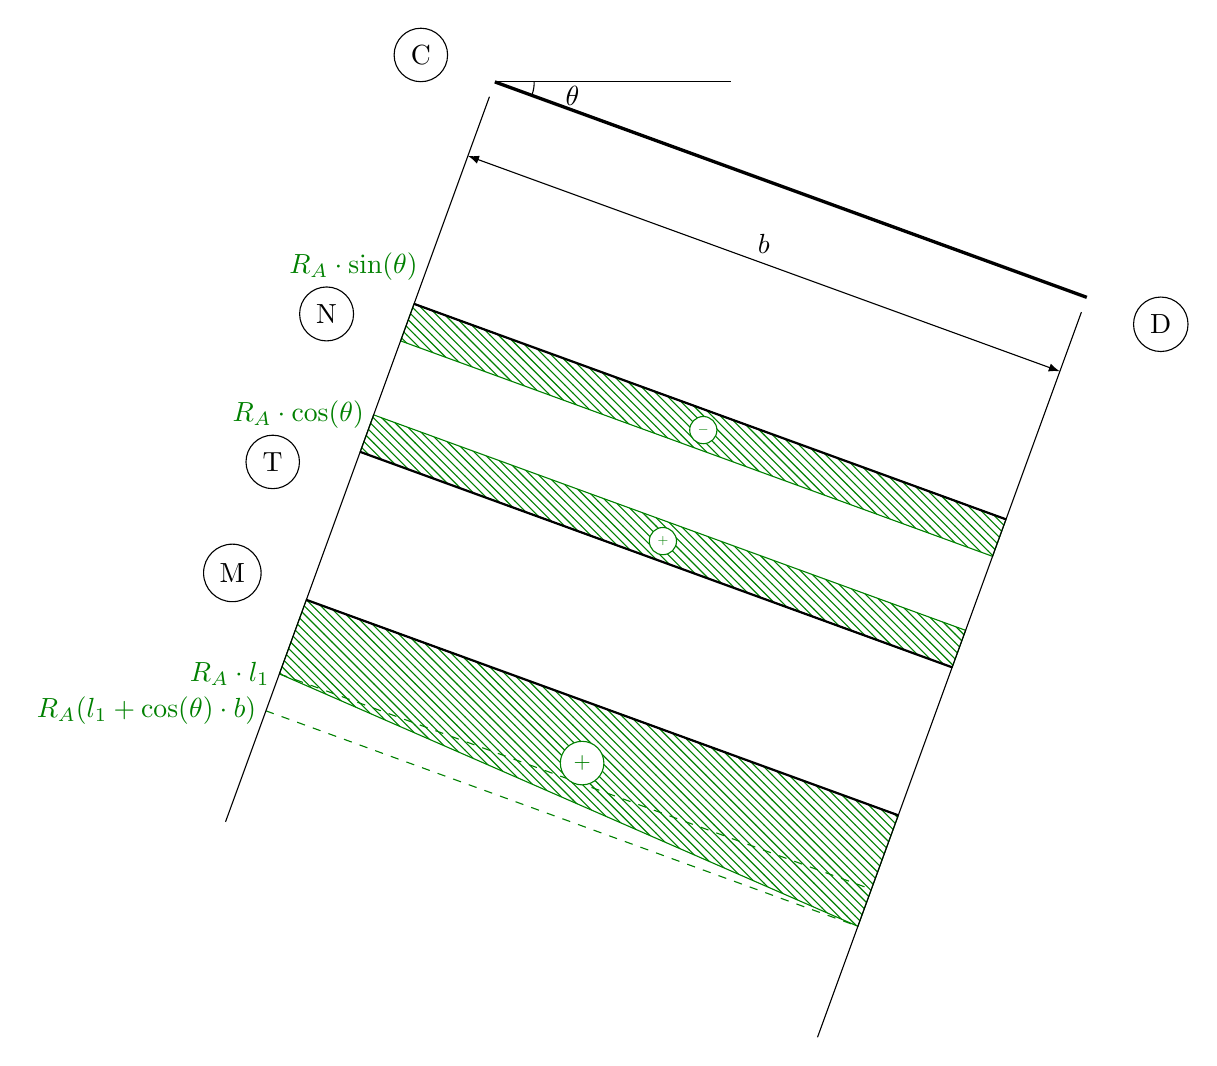
\begin{tikzpicture}[
	rotate=-\angle,
	label/.style={circle,draw},
	gFill/.style={Green, pattern=north west lines, pattern color=Green},
	arrow/.style={latex-latex},
	inSymb/.style={Green, fill=white, circle, draw}
	]
	
	\coordinate (C) at (0, 0);
	\coordinate (D) at (8, 0);
	
	\draw[very thick] (C) -- (D);
	\node [label] at ($(C) + (-1,0)$) {C};
	\node [label] at ($(D) + (1, 0)$) {D};
	
	% Draw angle
	\begin{scope}
		\coordinate (C1) at ({3*cos(\angle)}, {3*sin(\angle)});
		\coordinate (C2) at (2, 0);
		\draw (C) -- (C1);
		\node at ($(C) + ({\angle/2}:10mm)$) {$\theta$};
		\path[clip] (C) -- (C1) -- (C2);
		\draw (C) circle (5mm);
	\end{scope}
		
	\draw [arrow] ($(C) - (0, 1)$) -- ($(D) - (0, 1)$) node[midway, above] {$b$};
	
	\coordinate (N1) at ($(C) - (0, 3)$);
	\coordinate (N2) at ($(D) - (0, 3)$);
	\coordinate (N3) at ($(N2) - (0, .5)$);
	\coordinate (T1) at ($(N1) - (0, 2)$);
	\coordinate (T2) at ($(N2) - (0, 2)$);
	\coordinate (T3) at ($(T2) + (0, .5)$);
	\coordinate (M1) at ($(T1) - (0, 2)$);
	\coordinate (M2) at ($(T2) - (0, 2)$);
	\coordinate (M3) at ($(M2) - (0, 1.5)$);
	
	% Normal
	\node [label] at ($(N1) - (1, .5)$) {N};
	\draw[gFill] (N1) rectangle ($(N2) - (0, .5)$);
	\draw[thick] (N1) -- (N2);
	\node [Green, anchor=east] at ($(N1) + (0, .5)$) {$R_A \cdot \sin(\theta)$};
	\node[inSymb, scale=.5] at ($(N1)!.5!(N3)$) {$-$};
	
	% Tallant
	\node [label] at ($(T1) - (1, .5)$) {T};
	\draw[gFill] (T1) rectangle (T3);
	\draw[thick] (T1) -- (T2);
	\node[Green, anchor=east] at ($(T1) + (0, .5)$) {$R_A \cdot \cos(\theta)$};
	\node[inSymb, scale=.5] at ($(T1)!.5!(T3)$) {$+$};
	
	% Moment
	\node [label] at ($(M1) - (1, 0)$) {M};
	\draw[gFill] (M1) -- ($(M1) - (0, 1)$) -- (M3) -- (M2) -- cycle;
	\draw[thick] (M1) -- (M2);
	\draw[Green, dashed] ($(M1) - (0, 1)$) -- ($(M2) - (0, 1)$);
	\node[Green, anchor=east] at ($(M1) - (0, 1)$) {$R_A \cdot l_1$};
	\draw[Green, dashed] ($(M1) - (0, 1.5)$) -- ($(M2) - (0, 1.5)$);
	\node[Green, anchor=east] at ($(M1) - (0, 1.5)$) {$R_A (l_1 + \cos (\theta) \cdot b)$};
	\node[inSymb, scale=.8] at ($(M1)!0.5!(M3)$) {$+$}; 
	
	
	\draw ($(C) - (0, .2)$) -- ($(M1) - (0, 3)$);
	\draw ($(D) - (0, .2)$) -- ($(M2) - (0, 3)$);
	\end{tikzpicture}
\end{document}